\chapter{Exercises with answers}

\begin{Exercise} [
  title={Coding sequence},
  difficulty={1},
  label={excs},
  origin={G. Valle}
 ]
 
 \begin{figure}[H]
  \centering
  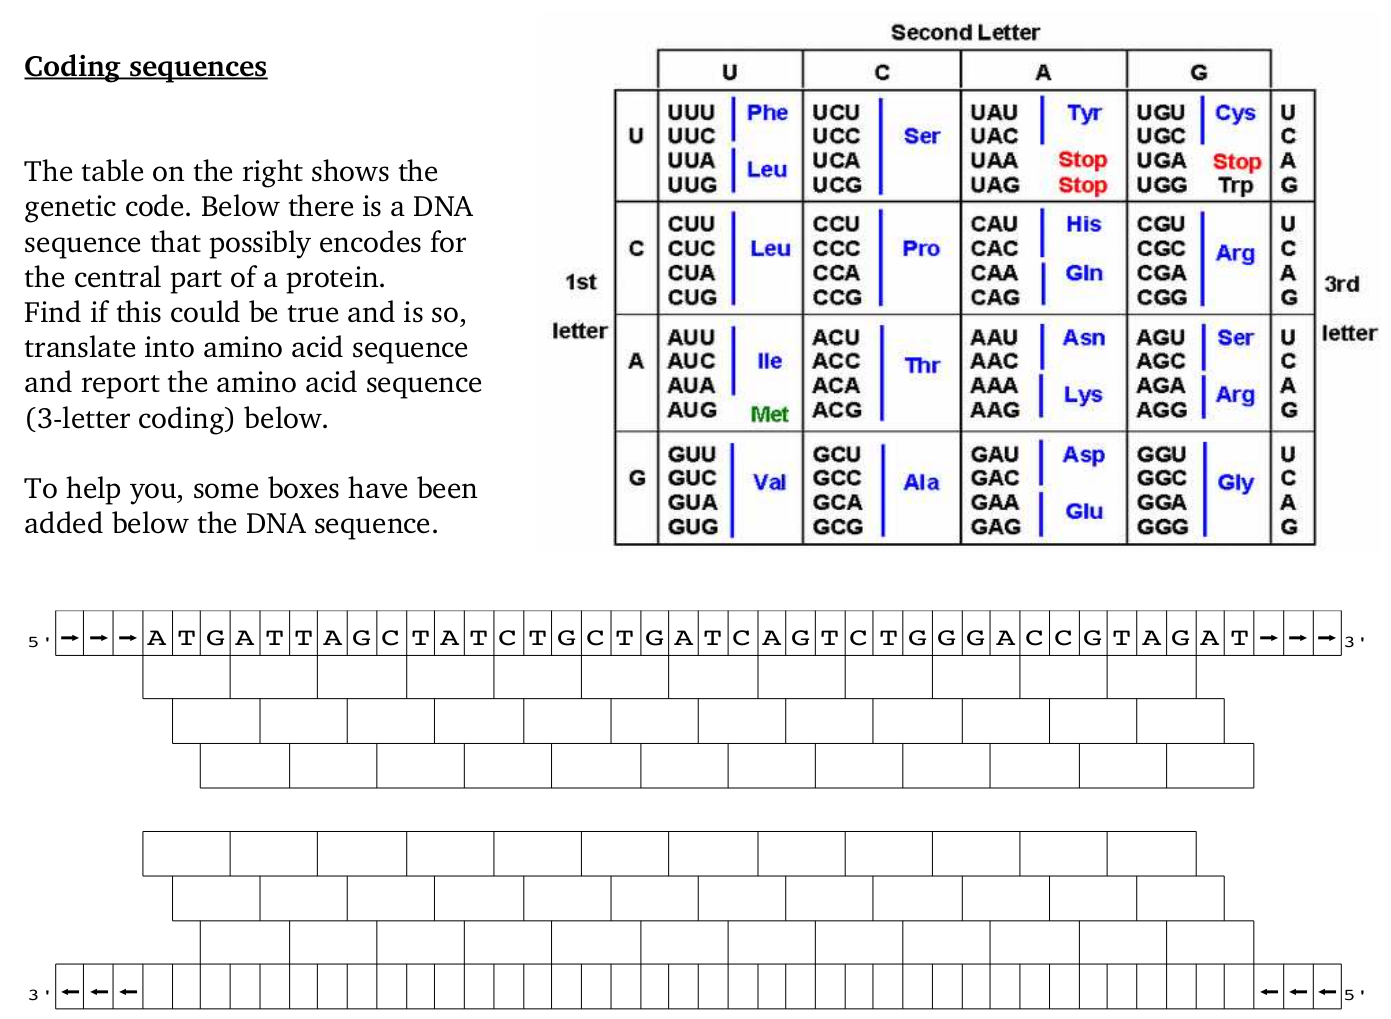
\includegraphics[scale=0.3]{Find_coding_sequence}
 \end{figure}

\end{Exercise}

\newpage

\begin{Answer} [
  ref={excs},
  number={1}
 ]
 
 \begin{figure}[H]
  \centering
  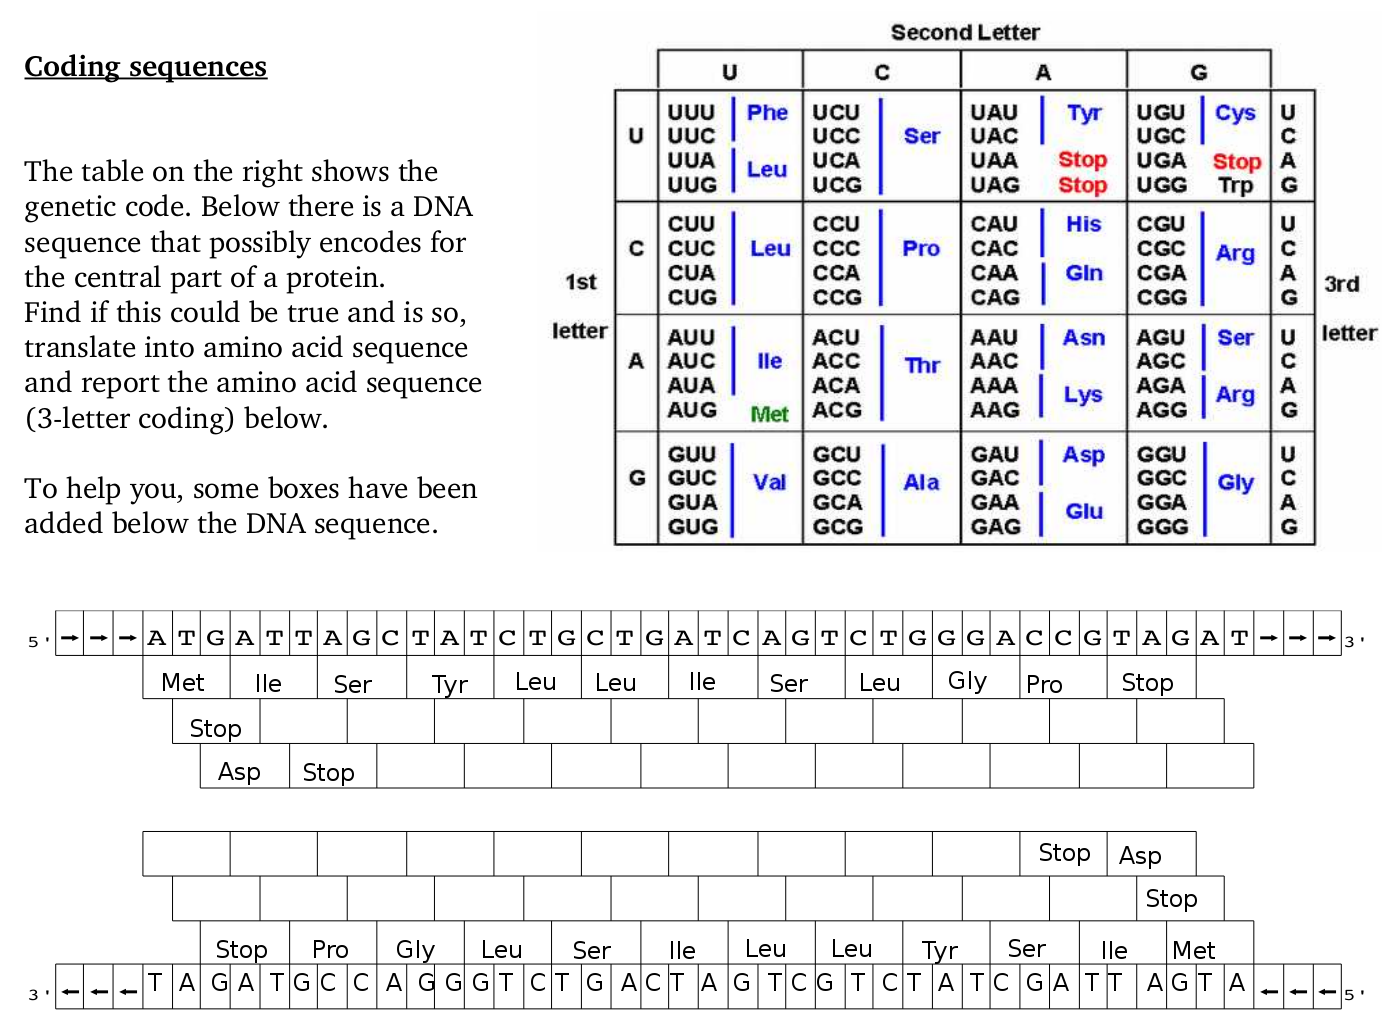
\includegraphics[scale=0.3]{Find_coding_sequence_sol}
 \end{figure}

\end{Answer}



\begin{Exercise} [
  title={Chromosomes},
  difficulty={1},
  label={ex1},
  origin={G. Valle}
 ]

  In adult human cells there are 46 chromosomes. De novo mutations are generally
very rare and we are not considering them in the following reasoning.
Answer \textbf{True} or \textbf{False}:

  \Question 23 chromosome are inherited from the mother and 23 from the father
  \Question Each chromosome of a child must have an identical copy in one of the
2 parents
  \subQuestion Explain why
\end{Exercise}

\begin{Answer} [
   ref={ex1},
   number={1}
 ]

  \Question True
  \Question False
  \subQuestion The second statement is wrong because of the crossing over

\end{Answer}


\begin{Exercise} [
  title={Genomes and genes},
  difficulty={1},
  label={ex2},
  origin={G. Valle}
 ]

  Approximately, how big is the genome and how many genes are there...

  \Question In a bacterium like \textbf{E. Coli}
  \Question In a simple eukaryote like \textbf{yeast}
  \Question In humans

\end{Exercise}

\begin{Answer} [
  ref={ex2},
  number={2}
 ]

  \Question Genome size: 100 Mbp. Number of genes: 19000 (27\% encoding)
  \Question Genome size: 13 Mbp. Number of genes: 6000 (70\% encoding)
  \Question Genome size: 3000 Mbp. Number of genes: 23000/25000 (1.5\% encoding)

\end{Answer}

\begin{Exercise} [
  title={Enzyme},
  difficulty={1},
  label={ex3},
  origin={G. Valle}
 ]

  Answer the questions.

  \Question How is called the enzyme that duplicate the DNA?
  \Question How is called the enzyme that transcribes DNS into RNA?
  \Question How is it called the biological structure where proteins are
synthesized?
\end{Exercise}

\begin{Answer} [
  ref={ex3},
  number={3}
 ]

  \Question DNA Polymerase
  \Question RNA Polymerase
  \Question Ribosome
\end{Answer}

\begin{Exercise} [
  title={Smith and Waterman algorithm},
  difficulty={1},
  label={exSW},
  origin={G. Valle}
 ]
 
 Consider the following two sequences:

 \begin{itemize}
  \item \texttt{DFTLNL}
  \item \texttt{EYSHMC}
 \end{itemize}

 Simulate the Smith-Waterman algorithm using the PAM240 and a gap penalty of
 4 points, both for starting and extending the gap.
 Finally, report the two aligned sequences below and the final score of the
 alignment.

 \begin{figure}[H]
  \centering
  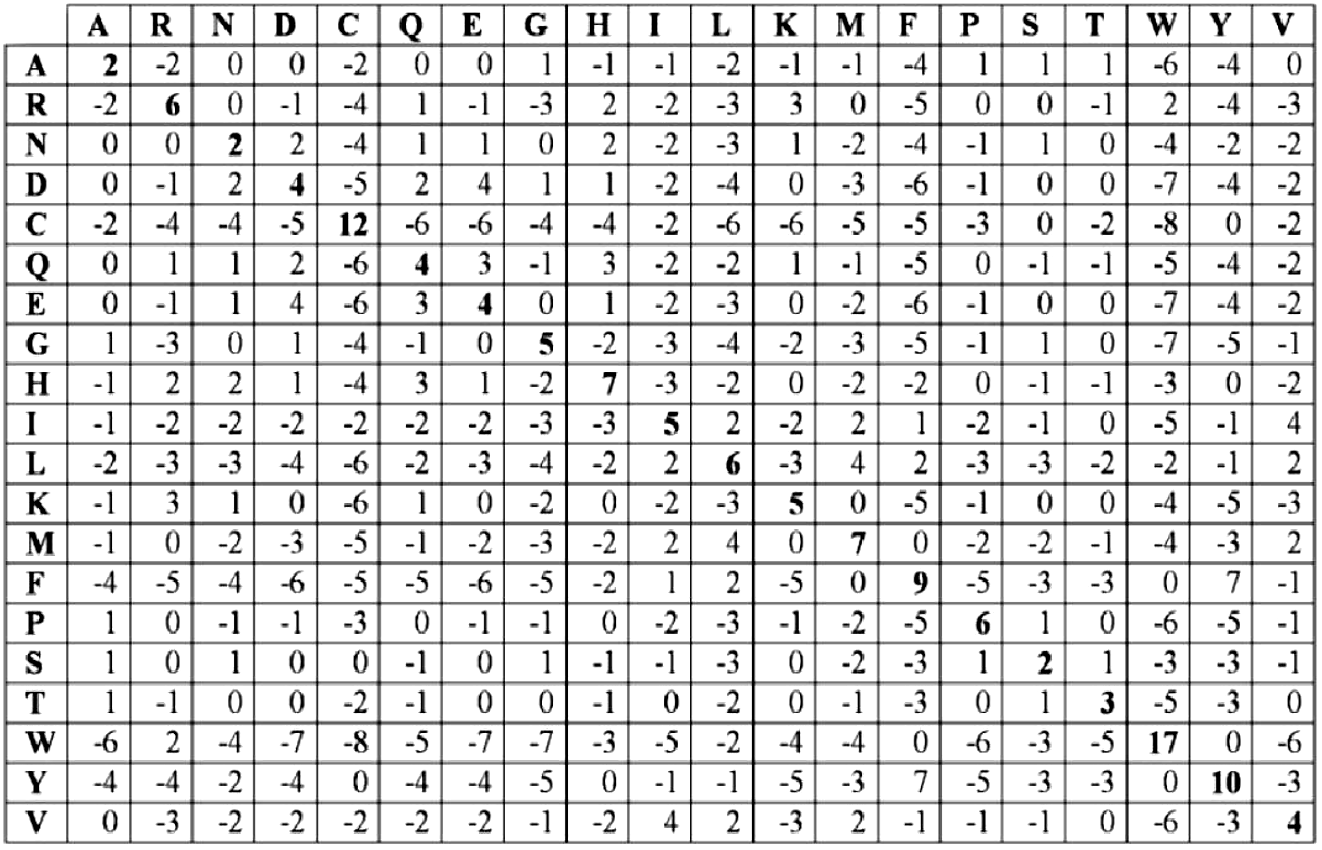
\includegraphics[scale=0.3]{PAM240}
 \end{figure}

\end{Exercise}

\newpage

\begin{Answer} [
  ref={exSW},
  number={4}
 ]
 
 The scoring matrix obtained by applying the algorithm is the following: 

 \begin{figure}[H]
  \centering
  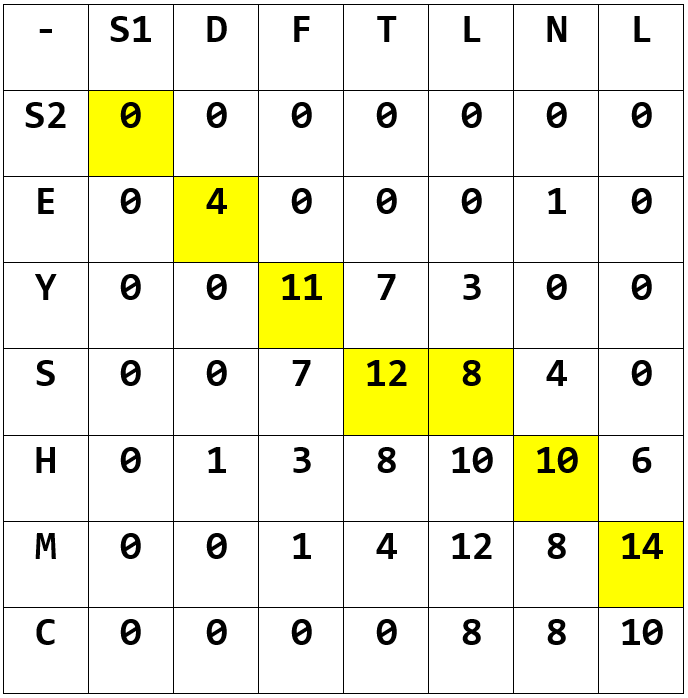
\includegraphics[scale=0.3]{matrix_ex}
 \end{figure}

 The \textbf{final alignment} is:

 \begin{figure}[H]
  \centering
  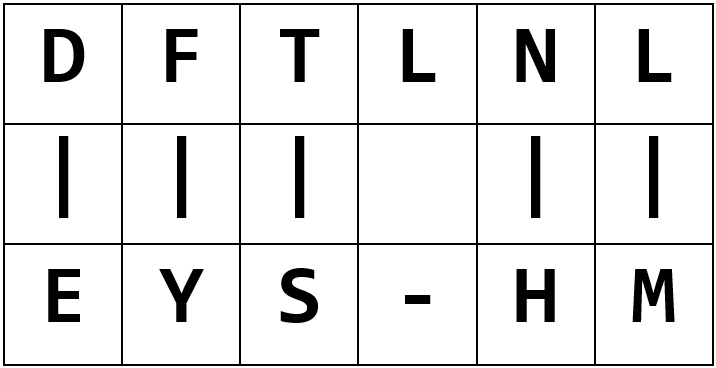
\includegraphics[scale=0.2]{alignment_ex}
 \end{figure}

 Thus, the \textbf{final score} is 14.

\end{Answer}

\section{Quiz}

\subsection{Flow of the genetic information}

\begin{Exercise} [
  title={Mitosis},
  difficulty={1},
  label={ex7},
  origin={G. Valle}
 ]

Answer \textbf{True} or \textbf{False}:

  \Question Mitosis is a process essential in the duplication of genetic
information of somatic cells.
Typically a diploid cell (2N) duplicates its DNA to become 4N, then the
chromosomes separate in two daughter diploid cells.

\end{Exercise}

\begin{Exercise} [
  title={Meiosis},
  difficulty={1},
  label={ex8},
  origin={G. Valle}
 ]

  \Question When we talk about DNA content in an eukaryotic cell, we refer to
N to indicate the DNA content.
Therefore we say that a haploid cell is 'N' and a diploid cell is '2N'.

Meiosis is a process essential in distributing genetic information in germinal
cells. What happens during  meiosis ?

Choose an alternative:

\begin{enumerate}
  \item During meiosis,  a diploid cell (2N) duplicates its DNA to become 4N,
then there are two cell divisions without DNA duplication, producing 4 haploid
cells called “gametes”, each with N chromosomes.
  \item The entire process of meiosis starts from a diploid cell (2N) that
divides itself into two haploid cells (N) called “gametes”, each with N
chromosomes.
\end{enumerate}

\end{Exercise}

\begin{Exercise} [
  title={Crossing-Over (1)},
  difficulty={1},
  label={ex9},
  origin={G. Valle}
 ]

Answer \textbf{True} or \textbf{False}:

  \Question Crossing over is a genetic process that is important in evolution
because it creates new mutations

\end{Exercise}

\begin{Exercise} [
  title={Crossing-Over (2)},
  difficulty={1},
  label={ex10},
  origin={G. Valle}
 ]

  \Question When does crossing over occurs?

Choose an alternative:

\begin{enumerate}
  \item It occurs during mitosis.
  \item It occurs during meiosis.
  \item It occurs at every cell duplication.
\end{enumerate}

\end{Exercise}

\begin{Exercise} [
  title={Eukaryotes},
  difficulty={1},
  label={ex11},
  origin={G. Valle}
 ]

Answer \textbf{True} or \textbf{False}:

  \Question Eukaryotes alternate haploid and diploid generations

\end{Exercise}

\begin{Exercise} [
  title={Haploidy},
  difficulty={1},
  label={ex12},
  origin={G. Valle}
 ]

Answer \textbf{True} or \textbf{False}:

  \Question The haploid status is predominant in most eukaryotes

\end{Exercise}

\begin{Exercise} [
  title={Diploidy},
  difficulty={1},
  label={ex13},
  origin={G. Valle}
 ]

Answer \textbf{True} or \textbf{False}:

  \Question Diploidy is important in evolution because it helps to eliminate
bad genes.

\end{Exercise}

\begin{Answer} [
   ref={ex7},
   number={7}
 ]

  \Question True

\end{Answer}

\begin{Answer} [
   ref={ex8},
   number={8}
 ]

  \Question 1

Typically, during meiosis,  a diploid cell (2N) duplicates its DNA to become
4N, then there are two cell divisions without DNA duplication, producing 4
haploid cells called “gametes", that are 1N.

\end{Answer}

\begin{Answer} [
   ref={ex9},
   number={9}
 ]

  \Question False

\end{Answer}

\begin{Answer} [
   ref={ex10},
   number={10}
 ]

  \Question 2

\end{Answer}

\begin{Answer} [
   ref={ex11},
   number={11}
 ]

  \Question True

It is true. For instance in mammals, there is the alternation between the
diploid phase (that is hugely predominant and multicellular) with the haploid
stage that is unicellular, represented by the egg and the spermatozoon.
The two haploid gametes join during fertilization to produce a diploid cell
that by means of many cell duplications (mitosis) will generate the fully
developed diploid organism.
Some specialized organs (gonads) are responsible to host the process of
gametogenesis where the haploid gametes are produced by meiosis.  

\end{Answer}

\begin{Answer} [
   ref={ex12},
   number={12}
 ]

  \Question False

\end{Answer}

\begin{Answer} [
   ref={ex13},
   number={13}
 ]

  \Question False

\end{Answer}
